\documentclass[12pt,PhD]{Thesis}



% ******** vmargin settings *********
\usepackage{vmargin} %This give you full control over the used page area, it maybe not the idea method in Latex to do so, but I wanted to reduce to amount of white space on the page
\setpapersize{A4}
%\setmargins{3.5cm}%			%linker Rand, left edge
%	  {1cm}%     %oberer Rand, top edge
%           {14.7cm}%		%Textbreite, text width
%           {23.42cm}%   %Texthoehe, text hight
%           {14pt}%			%Kopfzeilenhöhe, header hight
%           {1cm}%   	  %Kopfzeilenabstand, header distance
%           {0pt}%				%Fußzeilenhoehe footer hight
%           {2cm}%    	  %Fusszeilenabstand, footer distance   


%Defining text font profile
\usepackage{t1enc} % as usual




\usepackage[latin1]{inputenc} % as usual
\usepackage{times}	
\usepackage{mathcomp, subfigure}
\usepackage{amsmath}
\usepackage[pdftex]{graphicx}

\pagestyle{plain}
%\renewcommand{\topfraction}{0.99}
%\renewcommand{\bottomfraction}{0.99}
%\renewcommand{\textfraction}{0}


\dept{School of Physics and Astronomy}
\submitdate{2011}

\begin{document}
%Plan
%
\title{Measurements and Simulations of Impedance Reduction Techniques in Particle Accelerators}
\author{Hugo Alistair Day}
\principaladviser{Dr. Roger Jones}


\beforeabstract
\prefacesection{Abstract}
A review of the first two years of study are presented. These topics consist of; Simulations of coaxial wire measurements of the impedance of asymmetric devices, coaxial wire measurements of ferrite kicker magnets for use in the SPS and LHC and impedance studies of a number of potential collimator upgrades for the LHC, focusing on the phase 2 secondary collimators for the LHC. Also disucssed is future work towards completion of the PhD and a timetable of writing to ensure timely completion.
\afterabstract
\afterpreface


\tableofcontents

% What is new in the thesis:
% Wire measurements of asymmetric structures
% LMCI with SC and BB impedances - reconstructing Kell-Schnell diagram
% Simulations of wire measurements of structures
% Simulations of large structures (3m of magnets/kicker magnets)
%
%
%



\chapter{Introduction}
\section{Introduction}

The LHC collimation system is a key part of the machine protection system in the LHC. Due to extremely high stored beam and magnetic energy in the LHC [cite], amounting to some 160MJ of beam energy and 3GJ of stored magnetic energy, it is neccessary to keep close control on the losses experienced by the system. In the LHC this is done by a combination of monitoring the losses within the machine, carefully controlled losses by the collimation system, and a rigorous interlock system designed to dump the beam safely in the event of the development of dangerous behaviour by the circulating beam [LHC machine protection].

The collimation system in the LHC is a four-stage system, composed primarily of primary (TCP), secondary (TCS), and tertiary (TCT) collimators. These serve to scatter the particle halo, then further scatter and absorb the scattered particles. Further protection is provided by absorbers (TCLA), collimators at the injection regions (TCLI and TDI) and at the extraction region (TCDQA). In particular the TCTs are placed near the experimental IPs to protect the inner triplet magnets (used for final focusing of the beam before collision). In total the collimation system is broken down into two IRs; IR3 for betatron cleaning, in which there are:

\begin{enumerate}
\item{1 primary collimator}
\item{4 secondary collimators}
\item{4 absorbers}
\end{enumerate}

per beam and IR7 for momentum cleaning, which is composed of:

\begin{enumerate}
\item{3 primary collimators}
\item{11 secondary collimators}
\item{5 absorbers}
\end{enumerate}

per beam, with an additional 8 tertiary collimators (2 per experimental IP) per beam. In addition to the collimators at the injection and extraction region each beam is exposed to 44 different moveable collimators per circulation of the machine. The primary and secondary collimators presently all have a jaw material carbon reinforced graphite (conductivity $\sigma_{graphite} = 7 \times 10^{4} S m^{-1} $). This material was chosen due to the requirement for a robust jaw material (mechanically stable under large thermal shock) from a machine protection point of view, however not optimised from a beam impedance point of view.

The current collimation system has demonstrated to be exceptionally effective at it's job of providing machine protection to the LHC [cite Chamonix 2012 MP presentation], however it has been shown to be a limiting factor in the luminousity of the LHC due to the large contribution to the transverse beam coupling impedance by the primary, and especially the numerous secondary collimators in the system, which are also almost double the length of the primary collimators[cite]. 

\begin{figure}
\subfigure[]{
\label{fig:phase-1-col-longitudinal-rf}
}
\subfigure[]{
\label{fig:phase-1-col-sliding-contacts}
}
\label{fig:pĥase-1-rf}
\caption{Different components the impedance reduction measures in the phase 1 collimator design. \ref{fig:phase-1-col-longitudinal-rf} shows the longitudinal RF fingers, ensuring a good conducting path for the beam image currents, and \ref{fig:phase-1-col-sliding-contacts} shows the sliding RF contacts on the collimators jaw. These are intended to minimise the volume seen by the beam, thus making any cavity modes that may be excited by the beam at very high frequencies where the beam power spectrum is very small.}
\end{figure}

The phase 1 collimator (those presently (as of 2012) in place in the LHC) designs have a number of design features that are designed to reduce the beam coupling impedance of each device. Although the resistive wall contribution to the beam coupling impedance due to the poorly conducting jaw material is significant, the use of longitudinal RF fingers in the transition between the beam pipe to the collimator jaws and of a system of sliding contact fingers to isolate the beam from seeing the collimator vacuum tank (see Fig~\ref{fig:phase-1-rf} for more details). These function well as impedance reduction techniques, however have some limitations from a mechanical point of view. In particular, the sliding contacts have been suspected to be a significant producer of dust in the LHC due to the moving physical contact during collimator alignment [cite]. 

Due to these factors (high transverse impedance due to the resistive wall impedance and problems of dust due to sliding contacts) a phase 2 upgrade of the LHC collimation system has been proposed. This entails two components;

\begin{enumerate}
\item{The replacement of the current secondary collimators (the prime contributor to the large transverse impedance) by a phase 2 design using a good conducting material as the jaw material. There will be some loss of mechnical robustness but it is thought that this will not be detrimental to the requirements of machine protection with a suitable choice of material.}
\item{Replacing the existing sliding RF contacts with a contactless RF system (shown in Fig.~\ref{fig:rf-system-phase-2}). This is designed to remove the problem of dust caused by the sliding RF contacts in the phase 1 system by removing the moving physical contacts. This increase the volume of the cavity visible to the particle beam, decreasing the frequency of the lowest cavity modes. To counteract these new resonances, ferrite is placed in the cavity to decrease the resulting Q of the resonances.}
\end{enumerate}

\begin{figure}
\begin{center}
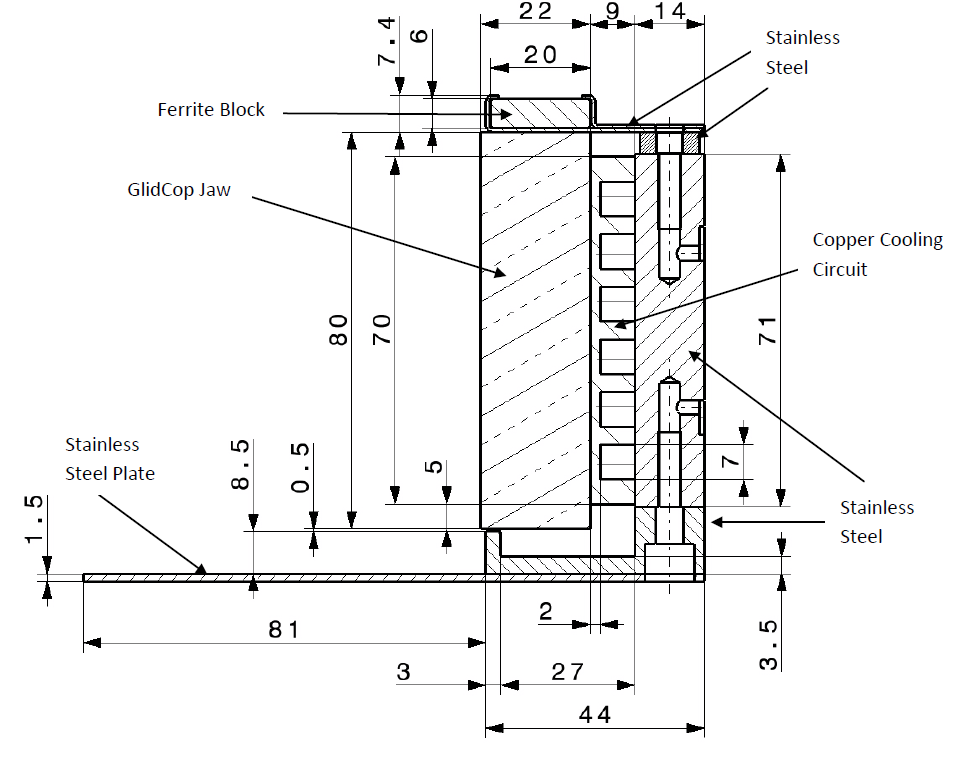
\includegraphics[width=0.7\textwidth]{LHC_Collimation_Upgrades/figures/cu-geo.png}
\end{center}
\label{fig:phase-2-rf-system}
\caption{The RF system for use in the phase 2 collimation system. The sliding RF contacts of the phase 1 design are replaced with a ferrite damping system. The RF contacts are removed, allowing the beam to see the entire RF cavity, causing resonances at lower frequencies. The Q of these resonances are decreased by the use of ferrite damping tiles.}
\end{figure}

In this chapter shall be presented an comparison of the different jaw materials proposed for use in the phase 2 secondary collimators, in particular a combination of jaw materials aimed at combining extremely robust materials with highly conductive metals, and the results of full 3D simulations of a TCTP collimator - a tertiary collimator for use in the LHC - which is incorporates the ferrite damping system in comparison to the sliding contacts of the phase 1 RF system. 



%
% Introduction to the new collimator design - Old collimator design, problems with sliding rails, new design, new material possibilities
% Material Evaluation - Comparison of CST simulations
% Whole collimator simulations of phase 2 secondary - Transverse and longitudinal modes with ferrite - compared to that from phase 1
% Sims in CST PS, GdFidl and HFSS
% Heating calculations also
%
%
%
%
%




\chapter{Wakefields and Impedance}
\section{Wakefields, Impedances and Beam Dynamics Effects}

\section{Theoretical Background of Wakefields and Impedances}

%
% Explaination of the concept of wakefields (the source and witness particle), oscillating electric fields
% induced by a charged particle. Longitudinal and Transverse wakefields

\begin{itemize}
\item{Wakes}
\begin{itemize}
\item{Introduction to the electromagnetic field of charged particle moving in free space}
\item{Field of a particle in a perfectly conducting pipe - method of image currents}
\item{Place a witness particle distance s behind source particle and deduce electric field as seen by this particle}
\item{normalise this by the source particle charge to give the wakepotential}
\item{And again by the source particle charge and current profile to acquire the loss factor}
\item{Longitudinal field predominantly}
\item{Introduce the Panowsky-Wenzel theorem covering transverse field - Transverse wakes}
\end{itemize}
\item{Impedance}
\begin{itemize}
\item{Firstly mention the commonality of frequency dependent material properties - ferrite permeability, permitivitty determined by conductivity/frequency in conductors/dielectrics/skin depth}
\item{Fourier transform of wakefield into the convolution of the beam current spectrum and the impedance}
\item{Again Panowsky-Wenzel for impedance}
\item{Discussion of the transverse impedance - in particular the general definition of an impedance (n-th order current interacting with an m-th order field)}
\item{Define dipolar/driving and quadrupolar/detuning impedance. In addition constant transverse impedance term}
\end{itemize}
\end{itemize}


\subsection{Resistive Wall Impedance}

\begin{itemize}
\item{Return to simple axisymmetric geometry concerning a finite conductivity of the wall}
\item{Derive in frequency domain - then have impedance. Give an example wakefield of a good conductor (copper), bad conductor (graphite), non-conductor (ferrite)}
\end{itemize}

\subsection{Geometric Impedance}
\begin{itemize}
\item{Derive the field pattern for a pillbox cavity - Oscillating fields with a characteristic frequency of some multiple of the lowest eigenfrequency}
\end{itemize}
\section{Examples of Effects}

\subsection{Beam-Induced Heating}
\label{sec:beam-heating-tctp}

As seen in Sec.~\ref{sec:imp-sims-tctp}, the longitudinal impedance of the phase 2 RF design indicates a significant number of beam impedance resonances below 1GHz. Although their contribution in the imaginary component of the beam coupling impedance is not significant enough to be of concern from a stability point of view, the resonances may present a problem from the point of view of beam-induced heating. To fully investigate both the effectiveness of the ferrite in damping the cavity resonances and to identify the locations of the power loss the phase 2 structure is investigated using the frequency domain code HFSS. 

For these simulations we simulate half of the structure (due to the reflective symmetry in the longitudinal plane), using alternatively perfect E-field (enforcing perpendicular electric fields at the boundary) and H-field (enforcing perpendicular magnetic fields at the boundary) boundary conditions at the symmetry plane to indentify and characterise the eigenmodes up to 2GHz (to cover the majority of the beam spectrum). The structure with and without ferrite is simulated to characterise the effect of the ferrite in damping the cavity modes. Simulations are carried out using the following parameters:

\begin{itemize}
\item{Using a 2$^{nd}$ order basis function solver to ensure good resolution of the fields for R/Q and localised loss calculations.}
\item{The ferrite is assumed to be 4A4, materials data is imported from an external data file and interpretted fit is used between data points. An analytical model (see [cite entry] for details).}
\item{We simulate using a single jaw seperation, in this case a half-seperation of 2mm. This is an extremely close jaw seperation, closer in fact than the TCTP collimator would be placed at, but similar to that that the phase 2 collimators would be placed at. This allows some prediction of a worst case scenario for the TCTP and also an analysis of the efficacy of the RF system for the type of operational parameters the phase 2 secondary collimators would be placed at.}
\item{The mesh was auto-generated by the HFSS mesh generator, and run for a convergence criteria of a 0.5\% convergence of the eigenmode frequency between two successive meshes with a 30\% refinement of the mesh between successive solutions.}
\end{itemize}

\begin{figure}
\begin{center}
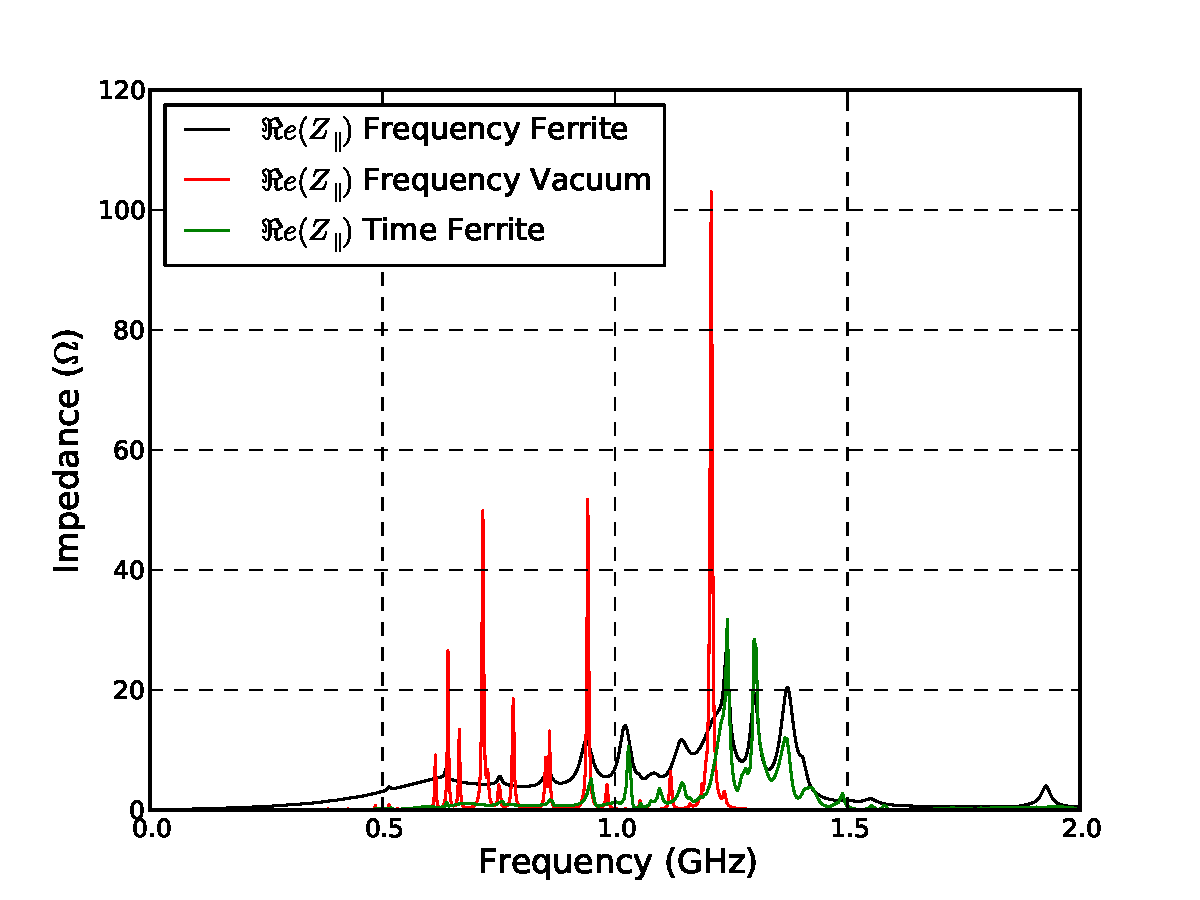
\includegraphics[width=0.7\textwidth]{LHC_Collimation_Upgrades/figures/longitudinal-impedance-tctp-ferr-freq-dom.pdf}
\end{center}
\label{fig:long-imp-tctp-freq}
\caption{The real component of the longitudinal impedance for the TCTP collimator as simulated by both the time and frequency domains for the case with and without ferrite damping tiles. The strong resonances present in the case without ferrite can be seen to be strongly damped when the ferrite tiles are added. However a substantial broadband component occurs in addition due to the broadened resonance peaks.}
\end{figure}

Here we shall evaluate the resonances as a whole, or a few key resonances from a heating point of view. For a complete listing of the eigenmodes please see App.~\ref{app:tctp-eigenmodes} for a complete breakdown of the TCTP eigenmode simulations. To have a comprehensive review of the heating we consider the following heating possibilities

\begin{itemize}
\item{A beam harmonic occuring exactly on the resonant frequency with a certain bunch profile. Here we consider gaussian and cos$^{2}$ bunch profiles. Parameters for a number of different beam operating modes (summarised in Tab.~\ref{tab:lhc-tctp-heating-para}) are considered.}
\item{Taking theoretical spectra for both 50ns and 25ns bunch spacings. In this case we consider the heating for both nominal operational parameters (1ns bunch length), running conditions from 2012 (bunch length between 1.2-1.4ns) and for HL-LHC parameters. These parameters are summarised in Tab.~\ref{tab:lhc-tctp-heating-para}. Different bunch profiles are considered - gaussian and cos$^{2}$ to account for high frequency lobes observed in measured beam spectra.}
\item{Using measured multi-bunch spectra for 50ns bunch spacing measured in the LHC. These measurements are for the beam from injection, through the ramp to squeeze and finally collisions.}
\end{itemize}

\begin{table}
\caption{The LHC operational parameters considered for heating estimates for the TCTP. Operational parameters include the nominal LHC parameters for 25ns bunch spacing, the peak operational intensity for 50ns bunch spacing used in 2012, and the two possible HL-LHC operational schemes, using both 25ns and 50ns bunch spacing. Here the bunch length is assumed to encompass the $4\sigma$ gaussian width.}
\label{tab:lhc-tctp-heating-para}
\begin{center}
\begin{tabular}{c | c | c | c | c }
Operational Mode & $\tau_{b}$ (ns) & $t_{bunch}$ (ns) & $N_{b}$ & $n_{bunches}$ \\ \hline
50ns, 2012 LHC Operation & 1.2 & 50ns & $1.7 \times 10^{11}$ & 1380 \\ \hline
25ns, Nominal LHC Operation & 1.0 & 25ns & $1.15 \times 10^{11}$ & 2808 \\ \hline
HL-LHC 25ns & 1.0 & 25ns & $2.0 \times 10^{11}$ & 2808 \\ \hline
HL-LHC 50ns & 1.0 & 50ns & $3.3 \times 10^{11}$ & 1380 \\ \hline
\end{tabular}
\end{center}
\end{table}

The heating estimates assuming on resonance beam harmonics can be seen in Tab.~\ref{tab:on-res-heating-tctp} for a variety of bunch lengths between 1-1.5ns assuming gaussian and cos$^{2}$ bunch distributions. The same data for the TCTP without the ferrite damping tiles can be seen in Tab.~\ref{tab:on-res-heating-tctp-no-ferr}. A number of things area immediately evident; 	The addition of the ferrite drastically reduces the power loss in the TCTP collimator, by a factor of $\approx$ 3. In addition, the consideration of the higher frequency lobes in the heating estimates for the TCTP is significant, as can be seen in Fig.~\ref{fig:tctp-heating-bunch-length-per-freq}. In this case the usefulness for the ferrites is clear.

\begin{table}
\label{tab:on-res-heating-tctp}
\caption{The power loss of a the TCTP collimator with ferrite for a number of operational modes in the LHC and HL-LHC assuming each cavity mode falls upon a beam harmonic. All losses are in watts using the parameters found in Tab.~\ref{tab:lhc-tctp-heating-para}}
\begin{center}
\begin{tabular}{c | c | c | c | c | c | c | c | c  }
$\tau_{b}$ (ns) & \multicolumn{2}{| c |}{50ns, 2012} & \multicolumn{2}{| c |}{25ns nominal} & \multicolumn{2}{| c |}{50ns, HL-LHC} & \multicolumn{2}{| c }{25ns, HL-LHC} \\ \hline
 & $P_{loss, g}$ & $P_{loss, c}$ & $P_{loss, g}$ & $P_{loss, c}$ & $P_{loss, g}$ & $P_{loss, c}$ & $P_{loss, g}$ & $P_{loss, c}$ \\ \hline
1.0 & 5.6 & 14.2 & 10.6 & 27.0 & 21 & 53.4 & 32.2 & 81.8 \\ \hline
1.1 & 3.8 & 10.2 & 7.2 & 19.6 & 14.4 & 38.8 & 22.0 & 59.0 \\ \hline
1.2 & 2.6 & 7.4 & 5.0 & 14.0 & 10.2 & 27.8 & 15.4 & 42.2 \\ \hline
1.3 & 2.0 & 5.4 & 3.6 & 10.0 & 7.2 & 20.0 & 11.0 & 30.4 \\ \hline
1.4 & 1.4 & 3.8 & 2.6 & 7.4 & 5.2 & 14.6 & 8.0 & 22.2 \\ \hline
1.5 & 1.0 & 2.8 & 2.0 & 5.4 & 3.8 & 10.8 & 5.8 & 16.4 \\ \hline
\end{tabular}
\end{center}
\end{table}

\begin{table}
\label{tab:on-res-heating-tctp-no-ferr}
\caption{The power loss of a TCTP collimator without the ferrite damping tiles for a number of operational modes in the LHC and HL-LHC assuming each cavity mode falls upon a beam harmonic. All losses are in watts using the parameters found in Tab.~\ref{tab:lhc-tctp-heating-para}}
\begin{center}
\begin{tabular}{c | c | c | c | c | c | c | c | c  }
$\tau_{b}$ (ns) & \multicolumn{2}{| c |}{50ns, 2012} & \multicolumn{2}{| c |}{25ns nominal} & \multicolumn{2}{| c |}{50ns, HL-LHC} & \multicolumn{2}{| c }{25ns, HL-LHC} \\ \hline
 & $P_{loss, g}$ & $P_{loss, c}$ & $P_{loss, g}$ & $P_{loss, c}$ & $P_{loss, g}$ & $P_{loss, c}$ & $P_{loss, g}$ & $P_{loss, c}$ \\ \hline
1.0 & 2.8 & 7.1 & 5.3 & 13.5 & 10.5 & 26.7 & 16.1 & 40.9 \\ \hline
1.1 & 1.9 & 5.1 & 3.6 & 9.8 & 7.2 & 19.4 & 11.0 & 29.5 \\ \hline
1.2 & 1.3 & 3.7 & 2.5 & 7.0 & 5.1 & 13.9 & 7.7 & 21.1 \\ \hline
1.3 & 1.0 & 2.7 &1.8 & 5.0 & 3.6 & 10.0 & 5.5 & 15.2 \\ \hline
1.4 & 0.7 & 1.9 & 1.3 & 3.7 &2.6 & 7.3 & 4.0 & 11.1 \\ \hline
1.5 & 0.5 & 1.4 & 1.0 & 2.7 & 1.9 & 5.4 & 2.9 & 8.2 \\ \hline
\end{tabular}
\end{center}
\end{table}

\begin{figure}
\label{fig:tctp-heating-bunch-length-per-freq}
\caption{The beam-induced heating of the TCTP with ferrite damping tiles for a number of different bunch lengths assuming both a gaussian and cos$^{2}$ distributions.}
\end{figure}

Considering the heating taking beam harmonics seperated the inverse of the bunch seperation (40$MHz$ for $t_{bunch} = 25ns$ and 20$MHz$ for $t_{bunch} = 50ns$) we acquire the results presented in Tab.~\ref{tab:heating-beam-harm-tctp-ferr} and Tab.~\ref{tab:heating-beam-harm-tctp-no-ferr} respectively, again for a variety of LHC operational parameters and assuming either a gaussian or a cos$^{2}$ longitudinal bunch profile. In this case it can be seen that the power loss for the ferrite case is larger than that experienced by the case without ferrite. This can be understood due to the fixed frequencies of the beam harmonics - if a high-Q resonance does not occur at or near a beam harmonic then the beam does not couple to the resonance. Due to the broad resonance peaks of the ferrite damped TCTP design the beam may couple to the resonance even if the resonance frequency of the cavity mode does not match the beam harmonic precisely due to the low-Q of the resonance.

\begin{table}
\label{tab:heating-beam-harm-tctp-ferr}
\caption{The power loss of a TCTP collimator with ferrite for a number of operational modes in the LHC and HL-LHC assuming beam harmonics spaced at the reciprocal of the bunch spacing. All losses are in watts using the parameters found in Tab.~\ref{tab:lhc-tctp-heating-para}}
\begin{center}
\begin{tabular}{c | c | c | c | c | c | c | c | c  }
$\tau_{b}$ (ns) & \multicolumn{2}{| c |}{50ns, 2012} & \multicolumn{2}{| c |}{25ns nominal} & \multicolumn{2}{| c |}{50ns, HL-LHC} & \multicolumn{2}{| c }{25ns, HL-LHC} \\ \hline
 & $P_{loss, g}$ & $P_{loss, c}$ & $P_{loss, g}$ & $P_{loss, c}$ & $P_{loss, g}$ & $P_{loss, c}$ & $P_{loss, g}$ & $P_{loss, c}$ \\ \hline
1.0 & 19.0 & 36.2 & 18.2 & 35.0 & 71.6 & 136.8 & 54.8 & 104.6 \\ \hline
1.1 & 14.8 & 29.2 & 14.2 & 28.0 & 56.2 & 110.0 & 42.8 & 85.0 \\ \hline
1.2 & 11.8 & 23.6 & 11.2 & 22.6 & 44.8 & 89 & 34.0 & 68.6 \\ \hline
1.3 & 9.6 & 19.2 & 9.0 & 18.4 & 36.2 & 72.6 & 27.4 & 55.6 \\ \hline
1.4 & 7.8 & 16.0 & 7.4 & 15.2 & 29.4 & 60.0 & 22.2 & 45.8 \\ \hline
1.5 & 6.4 & 13.2 & 6.0 & 12.6 & 24.2 & 50.0 & 18.4 & 38.0 \\ \hline
\end{tabular}
\end{center}
\end{table}

\begin{table}
\label{tab:heating-beam-harm-tctp-no-ferr}
\caption{The power loss of a TCTP collimator without ferrite for a number of operational modes in the LHC and HL-LHC assuming beam harmonics spaced at the reciprocal of the bunch spacing. All losses are in watts using the parameters found in Tab.~\ref{tab:lhc-tctp-heating-para}}
\begin{center}
\begin{tabular}{c | c | c | c | c | c | c | c | c  }
$\tau_{b}$ (ns) & \multicolumn{2}{| c |}{50ns, 2012} & \multicolumn{2}{| c |}{25ns nominal} & \multicolumn{2}{| c |}{50ns, HL-LHC} & \multicolumn{2}{| c }{25ns, HL-LHC} \\ \hline
 & $P_{loss, g}$ & $P_{loss, c}$ & $P_{loss, g}$ & $P_{loss, c}$ & $P_{loss, g}$ & $P_{loss, c}$ & $P_{loss, g}$ & $P_{loss, c}$ \\ \hline
1.0 & 2.8 & 7.1 & 5.3 & 13.5 & 12.1 & 25.0 & 16.1 & 40.9 \\ \hline
1.1 & 1.9 & 5.1 & 3.6 & 9.8 & 7.2 & 19.4 & 11.0 & 29.5 \\ \hline
1.2 & 1.3 & 3.7 & 2.5 & 7.0 & 5.1 & 13.9 & 7.7 & 21.1 \\ \hline
1.3 & 1.0 & 2.7 &1.8 & 5.0 & 3.6 & 10.0 & 5.5 & 15.2 \\ \hline
1.4 & 0.7 & 1.9 & 1.3 & 3.7 &2.6 & 7.3 & 4.0 & 11.1 \\ \hline
1.5 & 0.5 & 1.4 & 1.0 & 2.7 & 1.9 & 5.4 & 2.9 & 8.2 \\ 
\end{tabular}
\end{center}
\end{table}



\subsubsection{Location of Power Deposition}

\begin{figure}
\subfigure[]{

\label{fig:tctp-ferrite}
}
\subfigure[]{

\label{fig:tctp-long-rf-finger}
}

\label{fig:tctp-heat-loc}
\caption{The different thermally sensitive components of the TCTP collimator. \ref{fig:tctp-ferrite} shows the ferrite tiles, and \ref{fig:tctp-long-rf-finger} the longitudinal RF fingers.}
\end{figure}

Due to the poor cooling available in vacuum (cooled by radiative heating only. Although surrounded by a housing/in contact with surrounded components, the thermal contact between different components within the collimator is poor) it is important to know of the proportion of beam-induced power loss that is lost in thermally sensitive areas. These are areas where large increases in temperature can either lead to direct physical damage (as is the case with RF fingers) or may lead to a worsening physical condition of the collimator (if the ferrite tiles go above their Curie temperature). The components are highlighted in Fig.~\ref{fig:tctp-heat-loc}

The losses on or in different surfaces and volumes is calculated using the loss calculations within HFSS, and then normalised to the total losses in the TCTP structure for each mode. The produces a variety of losses depending on the field pattern of the mode. These are collated in App.~\ref{app:tctp-eigenmodes}. To provide a conservative estimate of the power load we take the highest proportions of power loss of all the modes and assume this is the case for all modes. The percentages for the total device, the ferrite tiles and the longitudinal RF fingers are shown in Tab.~\ref{tab:tctp-heating-loc}. 

\begin{table}
\label{tab:tctp-heating-loc}
\caption{The percentage of power loss lost in thermally sensitive components in the TCTP.}
\begin{center}
\begin{tabular}{c | c}
Component & Percentage of Power Loss \\ \hline
Whole Device & 100 \\ \hline
Ferrite Tiles & 5 \\ \hline
Longitudinal RF Fingers & 4 \\
\end{tabular}
\end{center}
\end{table}

\begin{table}
\label{tab:heating-ferr-power-load}
\caption{The power loss in the ferrite of the TCTP collimator. The most pessimistic of the losses estimated in Tab.~\ref{tab:on-res-heating-tctp} and Tab.~\ref{tab:heating-beam-harm-tctp-ferr} for the 1.0ns case. All losses are in watts using the parameters found in Tab.~\ref{tab:lhc-tctp-heating-para}}
\begin{center}
\begin{tabular}{c | c | c | c | c }
$\tau_{b}$ (ns) & 50ns, 2012 & 25ns nominal & 50ns, HL-LHC & 25ns, HL-LHC \\ \hline
 &  $P_{loss, c}$  & $P_{loss, c}$ &  $P_{loss, c}$  & $P_{loss, c}$ \\ \hline
1.0 & 1.8 & 1.7 & 6.8 & 5.2 
\end{tabular}
\end{center}
\end{table}


The thermal behaviour as a result of this power load can be analysed using design software such as ANSYS[cite]. The results of these thermal simulations can be seen in [cite F. Carra/M. Garlasche colwg meeting], a summary of which is given in Fig.~\ref{fig:tctp-ferrite-temp-rise}. The important figure of merit is in whether the temperature of the ferrite increases beyond its Curie temperature. For the TT2-111R, this 375$^{\circ}$C[cite data sheet]. The power loss for the worst cases of the nominal, HL-LHC and HL-LHC parameters without crab cavities (bunch length $0.5$ns rather than $1.0$ns) is considered, in this case with a factor of two margin of error included to be conservative (i.e. we assume double the power on the ferrite tiles), and it can be seen that the temperature increase for even the worst case results in the temperature being significantly below the Curie temperature for this material.

\begin{figure}
\begin{center}
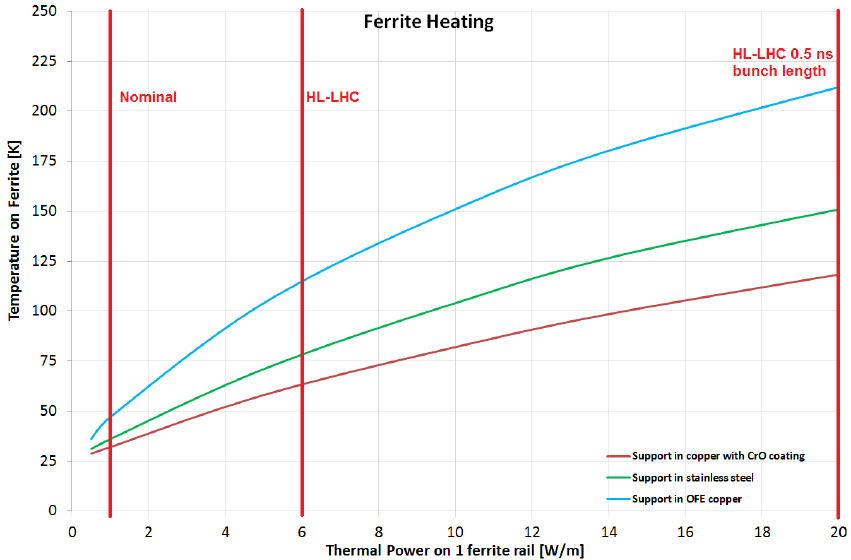
\includegraphics[width=0.75\textwidth]{LHC_Collimation_Upgrades/figures/temp_increase_tctp_col.png}
\end{center}
\label{fig:tctp-ferrite-temp-rise}
\caption{The temperature increase of the ferrite damping tiles in the TCTP collimator under a number of beam operating conditions and for a number of different jaw support materials. Plot taken from [cite Carra and Garlasche].}
\end{figure}

\subsection{Single Bunch and Coupled Bunch Instabilities}

\begin{itemize}
\item{Take references to introductory section on beam dynamics - longitudinal and transverse oscillations}
\item{Introduce bunch oscillation spectra - resonance diagrams for transverse motion, longitudinal spectra}
\item{Instabilities by resonance crossing, LMCI, TMCI, headtail instabilities, TCBI}
\item{Section on landau damping/transverse dampers? Other way to counter large impedances.}
\end{itemize}

\subsection{Example of LMCI with Broadband and Space Charge Impedances Studied with HEADTAIL}

%
% Theory of LMCI (potential well distortion and microwave instability)
% Simulations with BB, SC and BB/SC impedances
% Comparison of different impedances and their production of different stability criteria
%

\chapter{Bench Top Measurements of Beam Coupling Impedance}
%

Due to the sensitivity of the beam coupling impedance to the boundary conditions of the equipment used, it is necessary to utilise different measurement techniques to fully analyse the impedance of accelerator structures.

\section{Low Q-factor Impedances}

For structures that are expected to contain mostly low Q-resonances (i.e. resistive wall impedance) it is appropriate to use the coaxial wire method[ref], sometimes also called the stretched wire method. This method relies on the similarity of the electromagetic field profile due to an ultrarelativistic charged particle and that of a short electrical pulse sent along a coaxial wire. 

An moving charged particle produces an electromagnetic field in a arc transverse to its direction of motion, where the angle of the arc opening is proportinal to the relativistic factor of the particle $\gamma$. For an ultrarelativistic particle ($\gamma \leftarrow \infty$), the field becomes entirely perpendicular to the direction of motion. If we place a conductive wire along the same path we would expect the charged particle to take (in most cases this is well represented by a straight wire), a short electrical pulse sent along this wire would propogate in the TEM (transverse electrical and magnetic field) mode, producing a field profile similar to that emitted by the ultrarelativistic charged particle (see. Fig. \ref{fig:coax-part-profile})


\begin{figure}

\caption{Comparison of the electromagnetic field profile of a moving charged particle and a short time pulse propogating along a coaxial wire.}
\label{fig:coax-part-profile}
\end{figure}

\subsection{Classical Coaxial Wire Method}

The classical coaxial wire method, first proposed by V. Vaccarro in 1990 [ref], is a transmission method that measures the complex transmission coefficient of a DUT (Device Under Test) made up of the equipment whose impedance is to be measured and a coaxial wire passing through it. 

The experimental setup is as shown in Fig. \ref{fig:classic-coax}. Firstly the external circuit (i.e. everything not the DUT) is matched to the characteristic impedance of the coaxial line inside the DUT. This is done by measuring the reflection coefficient $\Gamma$ for the setup with only one port connected to the DUT and the other end terminated by an open connection. Knowing the characteristic impedance of the VNA and associated cables (typically $Z_{0} = 50\Omega$), we can easily calculate the characteristic impedance, $Z_{c}$, from the relation,

\begin{equation}
\Gamma = \frac{Z_{c} - Z_{0}}{Z_{c} + Z_{0}}.
\end{equation}

We then electrically match the characteristic impedance by adding resistors in series just before the DUT to resistively match the characteristic impedance of the VNA to that of the DUT. It is possible to use physical matching also using transition cones but these are costly, time consuming to construct and require new cones for each piecof equipment measured. And as can be seen in Fig. \ref{fig:matching-plot}, matching with a resistor is highly effective at removing the presence of reflections in coaxial measurements.

\begin{figure}

\caption{Experimental setup for a measurement of the beam coupling impedance using the classical coaxial wire method}
\label{fig:classic-coax}
\end{figure} 

\begin{figure}

\caption{An example of a reflection measurement made with and without a matching resistor. The faded line is the measurement without matching, the bold line that with. The reduction in the reflection can be seen.}
\label{fig:matching-plot}
\end{figure}

The value that we wish to measure to evaluate the beam coupling impedance of a device are the scattering parameters of the resulting circuit, in particular $S_{21}$, the normalised transmission parameter through the DUT. $S_{21}$ is calculated by taking the measured transmission parameter $S_{21,DUT}$ and dividing it by the transmission parameter through a reference line of the same physical length as the DUT,

\begin{equation}
S_{21} = \frac{S_{21,DUT}}{S_{21,REF}}
\end{equation}.

The effect of this is to correct the measured phase change in the DUT to be that only caused by the imaginary component of the beam coupling impedance.

There are subsequently a number of ways to evaluate the beam coupling impedance of the DUT depending on it's expected properties. For devices that are expected to have a either a small impedance, or those that are physically very short in length, it is possible to use the so called lumped impedance formula[ref];

\begin{equation}
Z = 2Z_{c} \frac{1-S_{21}}{S_{21}}
\end{equation}.

For distributed impedances, it is suitable to use the so called log formula (called so due to attenuation causing a log function to appear in the evaluation),

\begin{equation}
Z = -2Z_{c} ln \left( S_{21} \right)
\end{equation}.

For long components or measurements at very high frequencies there exists the improved log formula. This takes into account more completely the electrical length of the device, given by

\begin{equation}
Z = -2Z_{c} ln \left( S_{21}  \right) \left( 1 + j\frac{ln \left( S_{21}\right) }{2\Theta}  \right)
\end{equation}

where $\Theta = 2\pi \frac{L}{\lambda}$ is the normalised electrical length of the device, $L$ the length of the device, $\lambda$ the wavelength of the frequency of measurement. It is possible to see that the lumped impedance formula can be used when $\Theta \leq 1$, and the improved log formula becomes useful for $\Theta \geq 5$[erk's paper].




\subsection{Resonator Coaxial Wire Method}

An alternative method for measuring the beam coupling impedance is by using the so called resonator method. The setup for this method is similar to that of the classical coaxial wire method, except that the matching resistor network between the VNA and DUT is replaced by a weak capacitive coupling ($S_{11} < 0.5dB$) at both ends of the DUT. This then produces a structure which resonates at frequencies where the wavelength corresponds to the classical closed structure form,

\begin{equation}
\lambda = \frac{2L}{n}
\end{equation}

where $\lambda$ is the wavelength of the resonance, n the harmonic of the resonance and L the length of the device. 

The resonant method enables accurate measurement of the transmission losses due to the real longitudinal impedance. Additional advantages are that no matching is required, and a large number of mechanical uncertainties (electrical connections, consistency of calibration) can be avoided. However it can be seen that the frequency resolution is limited due to the length of the DUT so the method is not recommended as the only measurement method for structures expected to contain high-Q, narrowband resonances. It can however be used to corroborate the results obtained using the classical method.

For each resonancce peak, the loaded Q-factor and the frequency of the resonance are measured. For a weak coupling at both ends of the DUT, we can write the coupling coefficient k as

\begin{equation}
k = \frac{\left| S_{21} \right|}{1 - \left| S_{21} \right| }.
\label{eqn:coupling_coeff}
\end{equation}

The difference between the unloaded $Q$-factor, $Q_{0}$ , and the loaded $Q$-factor, $Q_{L}$, is a function of k. We can get an approximate correction by using the formula

\begin{equation}
Q_{0} = Q_{L} \left( 1 + k  \right).
\label{eqn:Q_correc}
\end{equation}

Subsequently the measured line attenuation (in Np/m) is then calculated

\begin{equation}
\alpha_{m} = \frac{\pi}{\lambda Q_{0}}.
\label{eqn:atten}
\end{equation}

Note that this attenuation includes both that from the beam coupling impedance due to the finite resistance of the wire material. We can estimate the attenuation due to the wire material as

\begin{equation}
\alpha_{w} = \sqrt{\pi \rho_{w} \epsilon f} \frac{1}{d ln D/d}
\label{eqn:wire_atten}
\end{equation}

where $\rho_{w}$ is the wire resistivity, $\epsilon$ the permitivitty, $f$ the frequency, $d$ the diameter of the inner conductor and $D$ the diameter of the outer conductor. At very low frequencies the finite skin depth of the inner conductor would also have to be taken into account. Using the corrected attentuation $\alpha = \alpha_{m} - \alpha_{w}$, the real longitudinal impedance per unit length can be found to be 

\begin{equation}
\Re e\left\{ Z \right\} = 2Z_{c} \alpha
\label{eqn:res_imp}
\end{equation}

\begin{figure}

\label{fig:res-resonancce-examples}
\caption{An example of the resonance pattern seen whilst performing measurements using the resonant method. Each peak corresponds to one data point in the final measurements.}
\end{figure}

To calculate the imaginary impedance using the resonant method involves a more involved calculation. In particular it is necessary to carry out measurements using the resonant method on a reference pipe of the same physical length to the DUT, either using physical measurements or a simulated measurement.

If we consider the complex impedance of the two measurements, $Z_{DUT}$ for the DUT and $Z_{REF}$ for a perfectly conducting reference pipe, we can simplify them as

\begin{align}
Z_{DUT} & =  R + jX_{1}  =  Z_{1}e^{j \phi} \\
Z_{REF} & =  jX_{2}  =  Z_{2}e^{j.0}
\end{align}

where $R$ is the resistive component of the DUT impedance, $X_{1/2}$ the imaginary component of the impedance (DUT and reference pipe respectively), $\phi$ is the angle of DUT impedance projected onto a complex plane and $Z_{2} = \sqrt{R^{2} + X^{2}}$. If we consider a measured value depedent on the impedance, for example the transmission parameter $S_{21}$ at a resonance peak, we have the following relations

\begin{align}
S_{21}^{DUT} = S_{0}e^{j \left( \omega_{1}t + \phi \right)} \\
S_{21}^{REF} = S_{0}e^{k \left( \omega_{2}t \right)}
\end{align}

where $S_{0}$ is some normalised scalar, $\omega_{1/2}$ is the frequency of the resonance and $t = \frac{L}{c}$ . Thus for a pair of corresponding peaks from resonance measurements for which we have measured $\omega_{1}$ and $\omega_{2}$ we can equate $S_{21}^{DUT} = S_{21}^{REF}$ and thus show

\begin{equation}
\phi = t \left( \omega_{2} - \omega_{1} \right).
\end{equation}

Subsequently we can see that

\begin{equation}
X = Z_{DUT} sin \phi = R \frac {sin \phi}{cos \phi} = R tan \phi
\end{equation}

where $R = \Re e(Z)$.

\subsection{Transverse Impedance Measurements}

The above methods give a general impression of how to carry out coaxial wire measurements of the impedance of accelerator components. Directly applied as described they allow the measurement of the longitudinal impedance of a DUT. However, from a beam stability point of view it is often more interesting to look at the transverse imedance of a device. In particular it would be useful to have a method of determining the vertical/horizontal dipolar (or driving) impedance and the vertical/horizontal quadrupolar (detuning) impedance of any device. In this section we describe how do this for structures with top/bottom, left/right symmetry and then generalising to asymmetric structures, with illustration from simple examples evaluated using simulations.

To allow a complete explanation of how to verify the methods of measuring transverse impedances, let us first consider the general form of the $m$-th order ($m = 0, 1, 2,...$) longitudinal beam coupling impedance, given by [ref]

\begin{equation}
\bar{Z}_{m} = \frac{-1}{I^{2}} \int dV \mathbf{\bar{E}_{m}. \bar{J}_{m}^{*}}
\end{equation}

where $\bar{J}_{m}$ is the current density of the source. For a beam propogating along the z-axis with an offset a and moment $cos \left( m \theta \right)$,

\begin{equation}
\mathbf{\bar{J}_{m}} = \frac{I}{\pi a^{m +1} \left( 1 + \delta_{m0} \right)} \delta \left( r - a \right) cos \left( m \theta \right) exp \left( j \left( \omega t - k z  \right) \right) \mathbf{e_{z}}.
\end{equation}

The electromagnetic field associated with a given current source $\mathbf{\bar{J}_{m}}$ is $\left( \mathbf{\bar{E}_{m}}, \mathbf{\bar{H}_{m}} \right)$. 

What can be seen is that any different azimuthal components of the $m$-th field of order n (i.e. $sin \left( n\theta \right)$ and $cos \left( n\theta \right)$ terms) are neglected in this treatment. To allow the treatment of coupling between different azimuthal orders we can define a longitudinal beam coupling impedance $Z_{m,n}$ (where $m,n = 0, \pm 1, \pm 2, ... $)

\begin{equation}
Z_{m,n} = \frac{-1}{I^{2}} \int dV \mathbf{E_{m}. J_{n}^{*}}
\end{equation}

where

\begin{equation}
\mathbf{J_{m}} = \frac{I}{\pi a^{|m |+1}} \delta \left( r - a \right) exp \left(j m \theta \right) exp \left( j \left( \omega t - k z  \right) \right) \mathbf{e_{z}}.
\end{equation}

Importantly, this allows us to see that 

\begin{align}
\mathbf{\bar{J}_{0}} &= \mathbf{J_{0}} \nonumber \\
\mathbf{\bar{J}_{m}} &= \mathbf{J_{m}} + \mathbf{J_{-m}}.
\end{align}

From here we use the principle of superposition for electromagnetic fields, and thus can derive

\begin{align}
\bar{Z}_{0} &= Z_{0} \\
\bar{Z}_{x} &= \bar{Z}_{1} = Z_{1,1} + Z_{1,-1} + Z_{-1,1} + Z_{-1,-1} = kZ^{dip}_{x}\\
\bar{Z}_{x} &= \bar{Z}_{1} \text{(cos replaced with sin)}= Z_{1,1} - Z_{1,-1} - Z_{-1,1} + Z_{-1,-1} = kZ^{dip}_{y}\\
\bar{Z}_{m} &= Z_{m,m} + Z_{m,-m} + Z_{-m,m} + Z_{-m,-m}, m=1,2,...
\end{align}

From this start we will apply this two both two wire measurements and to displaced single wire measurements.

\subsubsection{Two Wire Measurements}

It is possible to directly measure the dipolar impedance of a device through the use of a two wire coaxial method. The measurement setup is identical to that of the single wire method, except that two wires, seperated by distance $\Delta$, are placed in the device, and a 180$^{\circ}$ hybrid is place between the wires and the VNA at both ends of the device. This setup is illustrated in Fig. \ref{fig:two_wire_measure}

\begin{figure}

\label{fig:twowiremeasure}
\caption{Measurement setup for measurements of the dipolar beam coupling impedance using the two wire setup for the classical coaxial wire method.}
\end{figure}

The measurements are done in the same way as described in the previous sections for either the classical transmission method or the resonator method. By using two wires each carrying a signal 180$^{o}$ out of phase with one another we produce a field pattern similar to a dipole and thus measure the dipole impedance in either the horizontal or vertical plane depending on the orientation of the two wires. 

What is directly measured is the longitudinal impedance of just the dipole impedance, as is to be expected from the Panofsky-Wenzel theorem (see Chap. \ref{chap:wake_imp} for further explanation). 

For two wire placed as positions $x = \pm a$, the current density is given by [ref]

\begin{align}
J & =  I \left( \delta \left( x - a \right) - \delta \left( x + a  \right) \right) \delta (y) exp \left( j \left( \omega t - kz \right) \right) \nonumber \\
& =  \frac{I}{\pi a} \displaystyle\sum\limits_{m=-\infty}^{\infty} exp \left(j \left( 2m +1 \right) \theta \right) exp \left( j \left( \omega t - kz \right) \right) \nonumber \\
& =  2\displaystyle\sum\limits_{m=-\infty}^{\infty} a^{|2m + 1 |} J_{2m + 1}.
\end{align}

The impedance is then

\begin{align}
Z & =  - \frac{1}{I^{2}} \int dV \left( 2\displaystyle\sum\limits_{m=-\infty}^{\infty} a^{|2m + 1 |} E_{2m + 1}  \right)  \left( 2\displaystyle\sum\limits_{n=-\infty}^{\infty} a^{|2n + 1 |} J_{2n + 1}^{*}  \right) \nonumber \\
& =  4 \displaystyle\sum\limits_{m,n} a^{|2m + 1 | + |2n + 1|} Z_{2m + 1, 2n+1} \nonumber \\
& =  \left(2a \right)^{2}\left( Z_{1,1} + Z_{-1,1} + Z_{1,-1} + Z_{-1,-1} \right) + O(a^{4}) \nonumber \\
& =  (2a)^{2}\bar{Z}_{x} + O(a^{4}). 
\end{align}

Again using the Panofsky-Wenzel theorem we can deduce that the transverse dipolar impedance $Z^{dip}_{x/y}$ is given by 

\begin{equation}
Z^{dip}_{x/y} = \frac{\bar{Z}_{x/y}}{k} = \frac{c}{\omega} \frac{Z}{\Delta^{2}}
\end{equation}

where $\Delta = 2a$ and $Z$ is the measured complex impedance.

\subsubsection{Structures with Top/Bottom, Left/Right Symmetry}

If we consider a source particle at at $x_{1} = a_{1}cos\theta_{1}, y_{1} = a_{1}sin\theta_{1}$ and a test particle at $x_{2} = a_{2}cos\theta_{2}, y_{2} = a_{2}sin\theta_{2}$, the source current density is

\begin{align}
J_{z} &= I\delta \left( x-x_{1} \right) \delta \left( y-y_{1} \right) exp \left( k \left( \omega t - kz \right) \right) \nonumber \\
          &=\displaystyle\sum\limits_{m=-\infty}^{\infty}a_{1}^{|m|}exp\left( -jm\theta_{1} \right) J_{m}
\end{align}

The impedance would therefore be

\begin{align}
Z = &\frac{-1}{I^{2}} \int dV \left( \displaystyle\sum\limits^{\infty}_{m=-\infty} a_{1}^{|m|} exp \left( jm\theta_{1} \right) E_{m}\right) \left( \displaystyle\sum\limits^{\infty}_{n=-\infty} a_{1}^{|n|} exp \left( jn\theta_{2} \right) J^{*}_{n}\right) \nonumber \\
   = &\displaystyle\sum\limits^{\infty}_{m,n=-\infty} a_{1}^{|m|} a_{2}^{|n|} exp\left( -jm\theta_{1} \right) exp\left( -jn\theta_{2} \right) Z_{m,n} \nonumber \\
   = &Z_{0,0} + \left( x_{1}- jy_{1} \right)Z_{1,0} + \left( x_{1} + jy_{1} \right)Z_{-1,0} + \left( x_{2} + jy_{2} \right)Z_{0,1} +  \left( x_{2} - jy_{2} \right)Z_{0,-1} \nonumber \\
      & +\left( x_{1} - jy_{1} \right)^{2}Z_{2,0} +  \left( x_{1} - jy_{1} \right)\left( x_{2} - jy_{2} \right)Z_{1,-1} + \left( x_{2} - jy_{2} \right) Z_{0,-2} \nonumber \\
      & +\left( x_{1} - jy_{1} \right)\left( x_{2} + jy_{2} \right)Z_{1,1} + \left( x_{1} + jy_{1} \right) \left( x_{2} - jy_{2} \right) Z_{-1,-1} \nonumber \\
      & +\left( x_{1} + jy_{1} \right)^{2}Z_{-2,0} + \left( x_{1} + jy_{1} \right)\left( x_{2} - jy_{2} \right) Z_{-1,1} + \left( x_{2} - jy_{2} \right)^{2}Z_{0,2} \nonumber \\
      & +O\left( \left(  x_{1},y_{1},x_{2},y_{2} \right)^{3} \right).
\label{eqn:gen_imp}
\end{align}

By applying Panofsky-Wenzel we see

\begin{align}
kZ_{x} =\frac{\partial Z}{\partial x_{2}} = & Z_{0,1} + Z_{0,-1} + \left( x_{1} - jy_{1} \right) Z_{1,-1} + 2\left( x_{2} - jy_{2} \right) Z_{0,-2} \nonumber \\
						&+ \left( x_{1} - jy_{1} \right) Z_{1,1} + \left( x_{1} + jy_{1} \right) Z_{-1,-1} + \left( x_{1} + jy_{1} \right) Z_{-1,1} + 2\left( x_{2} + jy_{2} \right) Z_{0,2} \nonumber \\
						& + O\left( \left( x_{1},y_{1},x_{2},y_{2} \right)^{2} \right) \nonumber \\
						= & Z_{0,1} + Z_{0,-1} + x_{1}\bar{Z}_{x} + jy_{1} \left( -Z_{1,-1} - Z_{1,1} + Z_{-1,-1} + Z_{-1,1} \right) \nonumber \\
						& + x_{2}\left( 2Z_{0,-2} + 2Z_{0,2}  \right) + jy_{2}\left( -2Z_{0,-2} + 2Z_{0,2}  \right) +  O\left( \left( x_{1},y_{1},x_{2},y_{2} \right)^{2} \right)
\end{align}

\begin{align}
kZ_{y} =\frac{\partial Z}{\partial y_{2}} = & jZ_{0,1} - jZ_{0,-1} - j\left( x_{1} - jy_{1} \right) Z_{1,-1} - 2j\left( x_{2} - jy_{2} \right) Z_{0,-2} \nonumber \\
						&+ j\left( x_{1} - jy_{1} \right) Z_{1,1} - j\left( x_{1} + jy_{1} \right) Z_{-1,-1} + j\left( x_{1} + jy_{1} \right) Z_{-1,1} + 2j\left( x_{2} + jy_{2} \right) Z_{0,2} \nonumber \\
						& + O\left( \left( x_{1},y_{1},x_{2},y_{2} \right)^{2} \right) \nonumber \\
						= & j\left(Z_{0,1} - Z_{0,-1} \right)+ y_{1}\bar{Z}_{y} + jx_{1} \left( -Z_{1,-1} + Z_{1,1} + Z_{-1,-1} + Z_{-1,1} \right) \nonumber \\
						& + y_{2}\left(- 2Z_{0,-2} - 2Z_{0,2}  \right) + jx_{2}\left( -2Z_{0,-2} + 2Z_{0,2}  \right) +  O\left( \left( x_{1},y_{1},x_{2},y_{2} \right)^{2} \right).
\end{align}

Two properties to note for later use are that

\begin{align}
\textbf{J}_{-m} \left( \omega \right) & = \textbf{J}_{m}^{*} \left( -\omega \right) \\
Z_{-m,-n} \left( \omega \right) & = Z_{m,n}^{*} \left( -\omega \right).
\end{align}

If we now assume a single wire rather than a source and test particle, such that $x_{1}=x_{2}=x_{0}, y_{1}=y_{2}=y_{0}$. This gives a source current density

\begin{align}
J & = I \delta \left( x-x_{0} \right)\delta \left( y-y_{0} \right) exp\left( j \left(\omega t -kz \right)\right) \nonumber \\
  & = \frac{I}{2\pi a} \delta \left( r-a \right)\displaystyle\sum\limits_{m=-\infty}^{\infty} exp\left( jm \left( \theta -\theta_{0} \right) \right) exp\left( jm \left( \theta -\theta_{0} \right) \right) exp\left( j \left( \omega t - kz \right) \right) \nonumber \\
  & = \displaystyle\sum\limits_{m=-\infty}^{\infty} a^{|m|}exp\left( -jm\theta_{0} \right)J_{m}.
\end{align}

We can then define $x_{0}=acos\theta_{0}, y_{0}=asin\theta_{0}$. Entering this into Eqn. \ref{eqn:gen_imp} gives

\begin{align}
Z &=&Z_{0,0} +  \left( x_{0} - jy_{0} \right) Z_{1,0} + \left( x_{0} + jy_{0} \right)  Z_{-1,0} + \left( x_{0} + jy_{0} \right) Z_{0,1} \nonumber \\
   &   &+ \left( x_{0} - jy_{0} \right) Z_{0,-1} + \left( x_{0} - jy_{0} \right)^{2} Z_{2,0} + \left( x_{0} - jy_{0} \right)^{2} Z_{1,-1} + \left( x_{0} - jy_{0} \right) ^{2}Z_{0,-2} \nonumber \\
   &   &+\left( x_{0} - jy_{0} \right) \left( x_{0} + jy_{0} \right) Z_{1,1} + \left( x_{0} + jy_{0} \right)\left( x_{0} - jy_{0} \right) Z_{-1,-1} + \left( x_{0} + jy_{0} \right)^{2}Z_{-2,0} \nonumber \\
   &   &+\left( x_{0} + jy_{0} \right)^{2} Z_{-1,1} + \left( x_{0} + jy_{0} \right)^{2}Z_{0,2} + O\left( \left(x_{0},y_{0} \right)^{2} \right) \nonumber \\
   &=&Z_{0,0} + x_{0}\left( Z_{1,0}+Z_{-1,0}+Z_{0,1}+Z_{0,-1} \right) +jy_{0} \left( -Z_{-1,0} + Z_{-1,0} + Z_{0,1} - Z_{0,-1} \right) \nonumber \\
   &   &+x_{0}^{2} \left(  Z_{1,-1}+Z_{1,1}+Z_{-1,-1}+Z_{-1,1} + Z_{2,0} + Z_{0,-2} + Z_{0,2} + Z_{-2,0} \right) \nonumber \\
   &   &+y_{0}^{2} \left(  -Z_{1,-1}+Z_{1,1}+Z_{-1,-1}-Z_{-1,1} - Z_{2,0} - Z_{0,-2} - Z_{0,2} - Z_{-2,0} \right) \nonumber \\
   &   &+2jx_{0}y_{0}\left( -Z_{2,0} - Z_{0,-2} + Z_{-2,0} + Z_{0,2} + Z_{-1,1} - Z_{1,-1} \right) \nonumber \\
   &=&Z_{0,0} + x_{0}\left( Z_{1,0}+Z_{-1,0}+Z_{0,1}+Z_{0,-1} \right) +jy_{0} \left( -Z_{-1,0} + Z_{-1,0} + Z_{0,1} - Z_{0,-1} \right) \nonumber \\
   &   &+x_{0}^{2} \left( \bar{Z}_{x} + Z_{2,0} + Z_{0,-2} + Z_{0,2} + Z_{-2,0} \right) \nonumber \\
   &   &+y_{0}^{2} \left( \bar{Z}_{y} - Z_{2,0} - Z_{0,-2} - Z_{0,2} - Z_{-2,0} \right) \nonumber \\
   &   &+2jx_{0}y_{0}\left( -Z_{2,0} - Z_{0,-2} + Z_{-2,0} + Z_{0,2} + Z_{-1,1} - Z_{1,-1} \right).
\label{eqn:gen_single_wire}
\end{align}

It can then be seen that if measurements are made with $x_{0} = 0$ and take different values of $y_{0}$ that one obtains data with a parabolic fit in the $y_{0}$ axis. Be fitting a curve to this we obtain constant (equal to the longitudinal impedance), linear and quadratic terms. Doing the same for $y_{0}=0$ allows us to derive two quadratic terms

\begin{align}
Z^{\perp}_{x} & = \left( \bar{Z}_{x} + kZ_{quad} \right)\frac{1}{k} =  Z^{dip}_{x} + kZ_{quad}\\
Z^{\perp}_{y} & = \left( \bar{Z}_{y} - kZ_{quad} \right)\frac{1}{k}= Z^{dip}_{y} - kZ_{quad} \\
\end{align}

where $Z_{quad}=\frac{1}{k}\left( Z_{0,2}+Z_{2,0}+Z_{0,-2}+Z_{-2,0}  \right) = \frac{2}{k}\left( Z_{0,2}+Z_{0,-2}  \right)$, representing the impedance due to the displacement of the test particle in an accelerator. As we can measure $\bar{Z}_{x/y}$ independently using the two wire method we can thus indepedently measure $Z_{quad}$ using a displaced single wire scan in both the x- and y-planes.

It can also be seen that

\begin{align}
Z^{\perp}_{x} + Z^{\perp}_{y} = \frac{1}{k}\left( \bar{Z}_{x} + \bar{Z}_{y} \right) = Z^{dip}_{x} + Z^{dip}_{y}
\end{align}

where $\bar{Z}_{x/y}$ can be measured independently which gives a method of obtaining confidence in the wire measurements.

\subsubsection{Asymmetric Structures}

If Eqn. \ref{eqn:gen_single_wire} is transformed from $\left( x,y \right)$ coordinates to $\left( a, \theta \right)$, the result is

\begin{align}
Z &=Z_{0,0} +a\left[ cos\theta \left( Z_{-1,0} + Z_{0,1} \right) +jsin\theta \left( Z_{-1,0} + Z_{0,1} \right)  cos\theta \left( Z_{1,0} + Z_{0,-1} \right) - jsin\theta \left( Z_{1,0} + Z_{0,-1} \right)\right] \nonumber \\
   &+a^{2}\left[ cos^{2} \left( Z_{1,1} + Z_{-1,-1} \right) + sin^{2} \left( Z_{1,1} + Z_{-1,-1} \right)\right] \nonumber \\
   &+a^{2}\left[ cos^{2} \left( Z_{2,0} + Z_{0,-2} +Z_{1,-1} \right) +2jsin\theta cos\theta\left( Z_{2,0} + Z_{0,-2} +Z_{1,-1} \right) \right] \nonumber \\
   & - a^{2}\left[sin^{2} \left( Z_{2,0} + Z_{0,-2} +Z_{1,-1} \right)\right] \nonumber  \\
   &+ a^{2}\left[ cos^{2} \left( Z_{-2,0} + Z_{0,2} +Z_{-1,1} \right) +2jsin\theta cos\theta\left( Z_{-2,0} + Z_{0,2} +Z_{-1,1}  \right) \right] \nonumber \\
   &+ a^{2}\left[sin^{2} \left( Z_{-2,0} + Z_{0,2} +Z_{-1,1}  \right) \right].
\end{align}

Grouping like terms this becomes
\begin{align}
Z   &=Z_{0,0} + a\left[ e^{-j\theta}\left( Z_{-1,0} + Z_{0,1} \right) +  e^{j\theta}\left( Z_{1,0} + Z_{-0,1} \right)\right] \nonumber \\
     &+a^{2}\left[ \left( Z_{1,1} + Z_{-1,-1} \right) + e^{-2j\theta} \left(  Z_{2,0} + Z_{0,-2} +Z_{1,-1} \right) + e^{2j\theta} \left( Z_{-2,0} + Z_{0,2} +Z_{-1,1} \right) \right] \nonumber \\
     &=A_{1} + ae^{-j\theta}A_{2} + ae^{-j\theta}A_{3}+ a^{2}e^{-2j\theta}A_{4} +a^{2}e^{2j\theta}A_{5} +  a^{2}A_{6}
\label{eqn:rot_gen}
\end{align}

where $A_{1} = Z_{0,0}$, $A_{2} = Z_{0,1}+Z_{-1,0}$, $A_{3} = Z_{0,-1}+Z_{1,0}$, $A_{4} = Z_{0,2}+Z_{-1,1}+Z_{-2,0}$, $A_{5} = Z_{2,0}+Z_{1,-1}+Z_{0,-2}$ and $A_{6}=Z_{1,1}+Z_{-1,-1}$. Taking the earlier definition of $Z_{quad}$ it can be deduced that

\begin{align}
Z_{quad} & = \left( A_{4}+A_{5}+A_{6} - \bar{Z}_{x} \right)\frac{1}{k} =\frac{ A_{4}+A_{5}+A_{6}}{k} - Z^{dip}_{x} \\  
	    & = \left( A_{4}+A_{5} - \frac{\bar{Z}_{x}- \bar{Z}_{y}}{2}\right)\frac{1}{k} =\frac{ A_{4}+A_{5}}{k} - \frac{Z^{dip}_{x}-Z^{dip}_{y} }{2}.
\end{align}

Consideration of Eqn. \ref{eqn:rot_gen} lets it be seen that

\begin{align}
 A_{4}+A_{5}+A_{6} & = \frac{Z\left( a,0 \right)+Z\left( a,\pi \right) - 2Z\left( 0,0 \right)}{2a^{2}} \\
 A_{4}+A_{5} & = \frac{Z\left( a,0 \right)+Z\left( a,\pi \right) - Z\left( a,\frac{\pi}{2} \right)-Z\left( a,\frac{3\pi}{2} \right)}{2a^{2}}
\end{align} 

\subsection{Measurements on Example Geometries}

In this section shall be presented a number of example analyses of coaxial wire measurements done on geometries exhibiting top/bottom, left/right symmetry and an asymmetric structure. 

\section{High Q-factor Impedances}

For high Q-factor impedances, such as cavity impedances, it is not appropriate to use a coaxial wire method to measure the impedance due to the large perturbation of the boundary conditions that it causes [ref Vaccaro coaxial method], in particular below the cut-off frequency of the connecting beam pipes. This is due to the presence of the coaxial wire reducing the cut-off frequency to 0Hz, thus allowing propogation losses at all frequencies rather than just above cut-off. To illustrate this, we can consider the total Q of a cavity to be related to the "trapped" cavity mode Q and the propogation losses as;

\begin{equation}
\frac{1}{Q_{total}} = \frac{1}{Q_{cavity}} + \frac{1}{Q_{prop}}
\end{equation}

Under excitation by a charged particle beam, propogation losses do not exist below the cutoff frequency and thus $Q_{prop} = 0$. However, the addition of the coaxial wire causes these propogation losses to occur at all frequencies. Importantly, the Q-factor of these propogation losses is of a similar magnitude or smaller than that of the cavity resonance, leading to a great distortion of the measured Q. Similarly, the perturbation of the conductive wire in the centre of the structure leads to a shift in the resonance frequency of the cavity modes. 

To illustrate this phenomena, a number of simulations have been carried out to compare the measurements using the coaxial wire method compared to the impedance as simulated using CST Particle Studio[ref]

\begin{figure}
\subfigure[]{
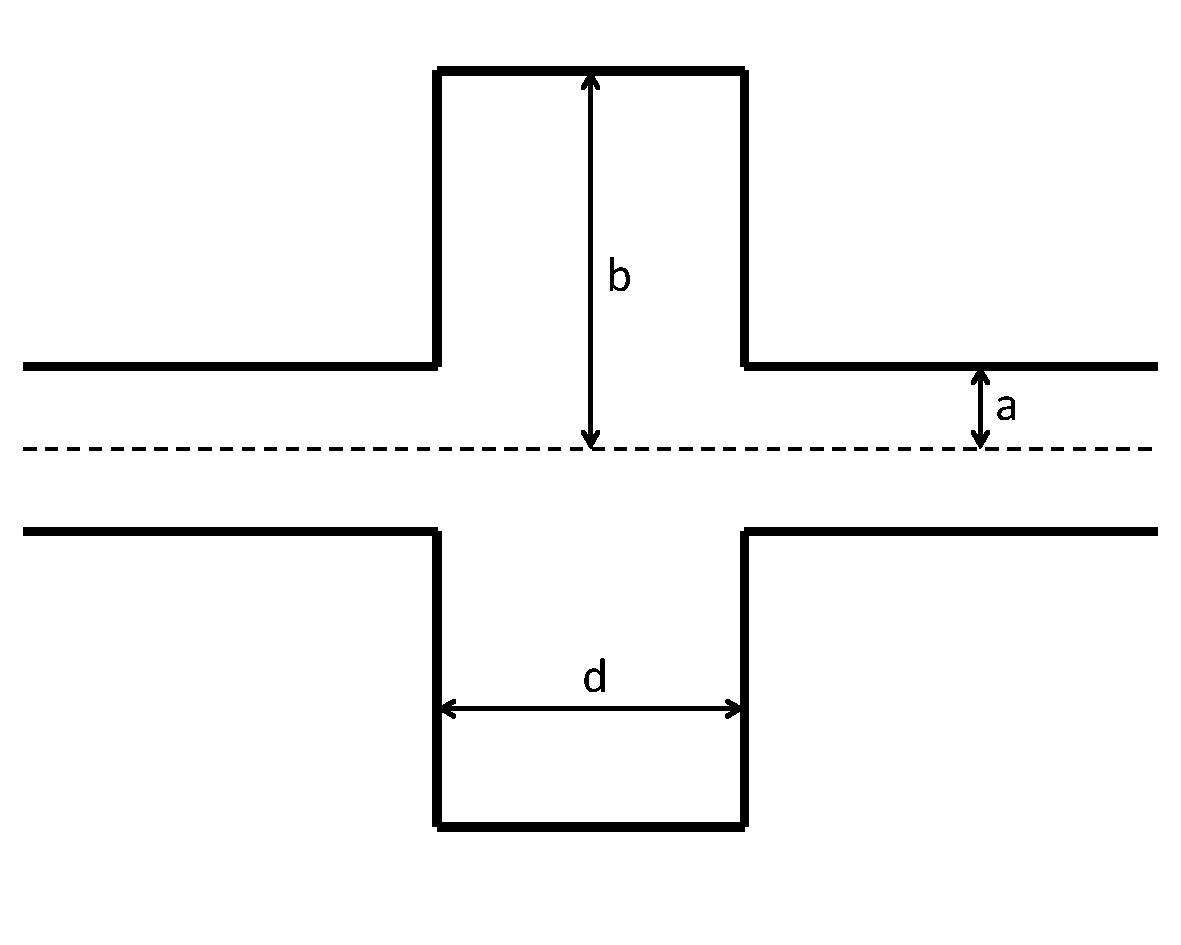
\includegraphics[width=0.5\linewidth]{figures/cavity_beampipe.pdf}
\label{fig:cavity_beampipe}
}
\subfigure[]{
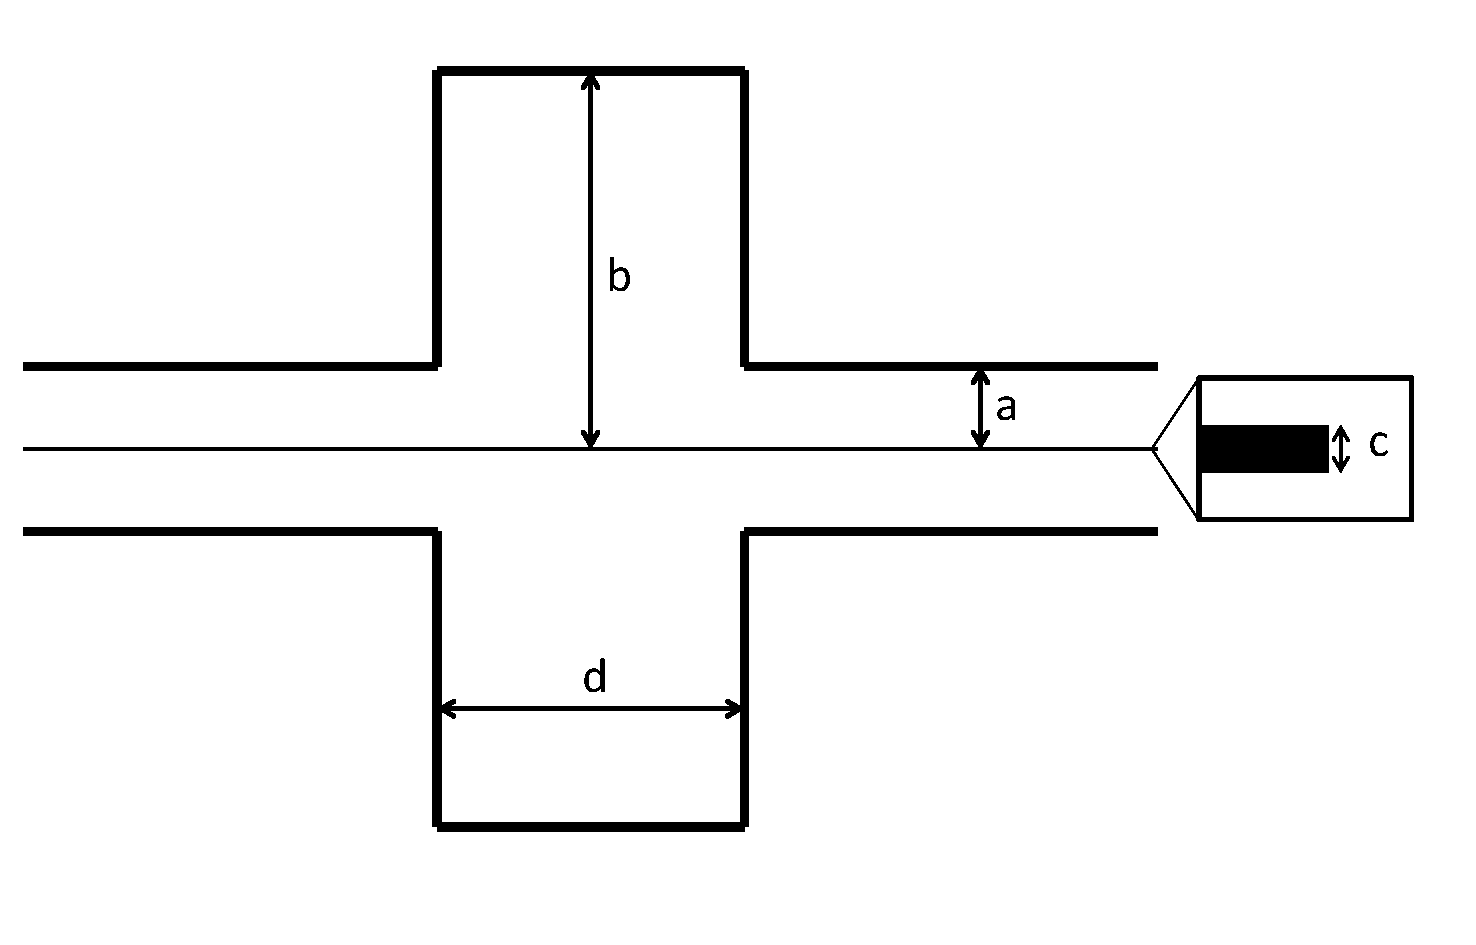
\includegraphics[width=0.625\linewidth]{figures/cavity_beampipe_coaxial.pdf}
\label{fig:cavity_beampipe_coaxial}
}
\caption{Comparison of the geometries of a cavity and attached beampipes \ref{fig:cavity_beampipe} without and \ref{fig:cavity_beampipe_coaxial} with the coaxial wire in place. Note the dimensions and that the dashed line in \ref{fig:cavity_beampipe} represents the rotational plane of symmetry}

\end{figure}

%
%  Things to do for high Q factor measurements
% - Simulation of transmission coefficients with and without coaxial wire
% - Comparison of impedance due to these resonances with time domain simulations
%
%
%
%
%
%
%
%
%
%



\chapter{Computational Simulations of Beam Coupling Impedance}
\section{Time Domain Simulations}

\begin{itemize}
\item{A VERY general introduction to time domain simulations codes. This is not a thesis of computational methods, only one thing you may do with them. Write this way}
\item{General experience - advantages of time domain methods (speed, memory footprint). Weaknesses (mesh resolution of structure, CPU limitation, long simulations times for high-Q resonances)}
\end{itemize}

\subsection{Direct Simulation of a Particle Beam}

\begin{itemize}
\item{Introduction to time domain code - simulation of a generic time signal, and the integration path}
\item{How we can subsequently simulate various types of impedance as a result}
\begin{itemize}
\item{Longitudinal - At various displacements}
\item{Transverse - dipolar/quadrupolar/constant with displacements of either the signal or the integration path, and subsequently taking gradient of resulting impedance}
\end{itemize}
\end{itemize}

\section{Frequency Domain Simulations}

\begin{itemize}
\item{Advantages of frequency domain - good resolution of structure by meshing, fast solution for individual modes, accurate for resonant structures. Weaknesses - Very memory intensive. Very time consuming to characterise structures over a large frequency ranges}
\end{itemize}

\subsection{Eigenmode Simulations}

\begin{itemize}
\item{To identify cavity modes of structures}
\item{Extract the resonant frequency and Q of cavity modes}
\item{fields on axis/off axis to extract R/Q, transverse R/Q}
\end{itemize}

\subsection{The Coaxial Wire Method by Simulation}
\begin{itemize}
\item{port solutions for driven modal simulations}
\item{Allow the extraction of S21}
\item{Evaluate as in previous section}
\end{itemize}

\subsection{Simulation of the particle beam}

\begin{itemize}
\item{Refer back to the nature of the EM field surrounding a charged particle beam (TEM-like)}
\item{We can enforce a TEM like profile on emitted radiation of a surface}
\item{With a TEM source with no wire - basically a particle beam}
\item{Evaluation as mentioned in Oleksey's paper}
\end{itemize}


\chapter{Beam Coupling Impedance Reduction Techniques}

\chapter{Case Studies}

\section{LHC Injection Kicker Magnet}

\begin{itemize}
\item{Introduction to the kicker magnet system}
\begin{enumerate}
\item{What are kicker magnets - Injection/Extractions systems}
\item{Why are they potentially a problem}
\end{enumerate}
\item{Explain the background of the LHC-MKI in particular}
\begin{enumerate}
\item{The original concern over heating, subsequent design of the beam screen}
\item{Observed problems with electrical breakdown of the beam screen, and subsequent removal of screen conductors}
\item{Recent observed heating in MKIs}
\end{enumerate}
\item{Summarise current state of the MKIs in the LHC - Beam screen layouts, two sets of kickers, one all of 15 screen conductors, one has one with 24}
\item{Comparison of the measurements and simulations of the LHC-MKI}
\begin{enumerate}
\item{Measurements of the Longitudinal BCI of the MKI - before and after bake out, with 15 and 19 screen conductors}
\item{Measurements of the transverse BCI of the MKI - if time just for interest and as a verification of the asymmetric method}
\end{enumerate}
\item{A breakdown of the impedance that we see in the MKI}
\begin{enumerate}
\item{Start with a simple c - core ferrite magnet}
\item{Add a ceramic tube}
\item{Add screen conductors in internal side - Brief interlude about the limitations this places on the magnet rise time due to creating a Faraday cage}
\item{Add the capacitive coupling - Different lengths of overlap to demonstrate that this controls the frequency of the resonances. Also lengths of the screen conductors for lower resonances}
\item{Add the ferrite damping rings - damp resonances of length of screen conductor - not(!) overlap}
\item{Hopefully show that this is the dominant cause of the resonances}
\end{enumerate}
\item{Summary of different beam screen designs - Where possible include discussion about the reduction of the voltage build up on each screen conductor}
\begin{enumerate}
\item{Screen conductors all of the same length with capactive coupling at one end - Show how increasing the number of screen conductors really helps to reduce the BCI}
\item{Screen conductors with a tapering of the length, with the longest at the side towards the ground plate and the shortest towards the HV plate}
\item{Alternating lengths of long and short screen conductors}
\item{Having the screen conductors in closed slots in the ceramic tube}
\item{The addition of small conducting spheres to the ends of the screen conductors to reduce the high fields at the conductor ends}
\item{Thicker ceramic at the capacitively coupled end of the beam screen to reduce the field gradient}
\item{Alternative beam screen design - Most screen conductor capactively coupled at both ends, with two connected to the beam pipe at one end. Aim to reduce the potential on all conductors by conductively connecting them at the capactively coupled end}
\item{Stepping the external metallization away from the ceramic tube at the ends of the screen conductors. The metallization will be removed and a conducting pipe placed there instead - different step out dstances are investigated}
\end{enumerate}

\item{Heating estimates for all of the above}
\begin{enumerate}
\item{Explain completely the methods of estimating the power losses here - bunch intensity, number of bunches, bunch length, distribution}
\item{Note the benefits of increasing the bunch length for the resonances with 15 screen conductors}
\item{Summary charts of the beam induced heating for the others, and plots illustrating how the changes in bunch length changes the power loss}
\item{Impedance profiles of all of the above - longitudinal predominantly}
\item{Some judgement on which is most appropriate for an impedance point of view}
\item{Comments on the improvements made to existing magnets already - 19 screen conductors}
\end{enumerate}
\end{itemize}
%
% Introduction to kicker magnet systems - PFNs and the materials normally used
% Risks of beam coupling impedance to the kicker magnet system
% Existing beam coupling impedance reduction - ceramic screen with conductive inserts. Limits of this (electrical breakdown)
% First - comparison of simulations to measurements
% Second - Proposals of improvements to the reduction measures - Rounded ends, changing strips arrangements
% Evaluation of new proposals - comparison of heat load (different methods of evaluating heat load (assume crosses resonance, or real spectrum)), explaination of 
% spectrum measurements and the differences bunch length and profile can make
%
%
%



\section{LHC Phase 2 Collimator Designs}
\begin{itemize}
\item{Introduction to the collimator upgrade project - Why are collimators important}
\begin{enumerate}
\item{The have two significant physical requirements - a rigid, sturdy material and must be placed very close to the beam}
\item{The first necessitated the use of graphite/carbon materials for the phase 1 collimators due to their survivability in the condition needed. The second means that the resistive wall impedance is very large}
\end{enumerate}
\item{Phase 2 collimator materials choice}
\begin{enumerate}
\item{Why a phase 2 collimator upgrade?}
\item{Summary of the material requirements and the available materials}
\item{Simple model used - simulations and comparison to analytical models}
\end{enumerate}
\item{TCTP Impedance Studies}
\begin{enumerate}
\item{What is the TCTP? Why do we need it?}
\item{Possibly designs}
\begin{itemize}
\item{Structure with RF fingers isolating the beam from the vacuum tank}
\item{Structure with a narrow connection between central cavity and vacuum tank - simulated with and without ferrite to demonstrate reduction in Q}
\end{itemize}
\item{Simulations Parameters and results}
\item{Heating estimates - using single bunch, multi-bunch, on resonance and equally spaced}
\item{Localisation of the heating - using both CST and HFSS}

\end{enumerate}
\end{itemize}
%
% Introduction to the new collimator design - Old collimator design, problems with sliding rails, new design, new material possibilities
% Material Evaluation - Comparison of CST simulations
% Whole collimator simulations of phase 2 secondary - Transverse and longitudinal modes with ferrite - compared to that from phase 1
% Sims in CST PS, GdFidl and HFSS
% Heating calculations also
%
%
%
%
%




\bibliographystyle{IEEEtran}
\bibliography{general_bibliography}

\end{document}
